\documentclass{beamer}

% Required packages and libraries
\usetheme{Madrid}
\usepackage{tikz}
\usepackage{multirow}
\usepackage{circuitikz}
\usetikzlibrary{calc}
\usepackage{color, colortbl}
	
\definecolor{Gray}{gray}{0.9}
\definecolor{LightCyan}{rgb}{0.88,1,1}

\title{Flip-flops \& Race-around Problems}
\author[FT, SIS]{Farhan Tanvir \\ 1805073 \\ Shehabul Islam Sawraz \\ 1805088}
\institute[BUET]
{
  Department of Computer Science and Engineering\\
  Bangladesh University of Engineering and Technology
}
\date{\today}

\AtBeginSection[]
{
  \begin{frame}
    \frametitle{Checkpoint}
    \tableofcontents[currentsection]
  \end{frame}
}

\begin{document}

\begin{frame}
    \maketitle
\end{frame}

\begin{frame}{Table of Contents}
    \tableofcontents
\end{frame}

\section{Introduction}
\begin{frame}{Before We Start!!!}
    \setbeamercovered{transparent}
    \begin{itemize}
        \item Before we dive into the discussions of Flip-flops, let's go for a quick introduction of it!
        \pause
        \item And for that, we will need to know about one important concept first! 
    \end{itemize}
\end{frame}

\begin{frame}{Sequential Circuits}
    \begin{itemize}
        \item We know, pretty much in everywhere, output depends on input.
        \pause
        \item Putting it more formally in case of circuits... \textcolor{blue}{present output depends on present input.}
        \pause
        \item \textbf{But output of sequential circuits depend on past output too!!!}
    \end{itemize}
\end{frame}

\begin{frame}{Sequential Circuits (contd.)}
    \begin{itemize}
        \item That brings an important point: we need to \alert{store} the past output somewhere.
        \pause
        \item For that, we need storage devices. 
        \pause
        \item And here is where \textbf{Flip-flop} comes in play.
        \pause
        \item This whole thing is also known as \textcolor{blue}{storing the state of our circuit.}
    \end{itemize}
\end{frame}

\begin{frame}{Two Important Questions}
\begin{enumerate}
    \item What does Flip-flop do?
    \begin{itemize}
        \item It stores and updates the state of our circuit
    \end{itemize}
    \pause
     \item How does it know when to update the state?
    \begin{itemize}
        \item It updates upon receiving a signal, whom we refer to as \textcolor{blue}{clock}
        \break
        \begin{figure}
            \centering
            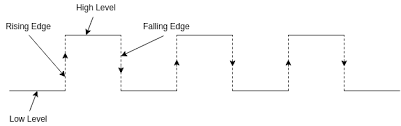
\includegraphics[width=0.8\textwidth]{download.png}
            \label{fig:my_label}
        \end{figure}
    \end{itemize}
\end{enumerate}
\end{frame}

\section{Types}
\begin{frame}{Types of Flip-flops}
    \begin{itemize}
        \item SR (Set-Reset FF)
        \item D (Delay FF)
        \item T (Toggle FF)
        \pause
        \item \textbf{JK (Jack Kilby FF)}
    \end{itemize}
\end{frame}

\section{Truth Table}
\setbeamercovered{transparent}
\begin{frame}{Truth Table for JK Flip-flop}
    \newcolumntype{g}{>{\columncolor{Gray}}c}
    \begin{table}
        \centering
        \begin{tabular}{|g|g|c|c|c|}
            %\cline{1-4}
            \hline
            J & K & $Q_{n-1}$ & $Q_n$ & Mode \\
            %\cline{1-4}
            \hline
            \pause
            
            0 & 0 & 0 & 0 & \multirow{2}{*}{Hold/Store} \\
            \cline{1-4}
            0 & 0 & 1 & 1 & \\
            %\cline{1-4}
            \hline
            \pause
            
            0 & 1 & 0 & 0 & \multirow{2}{*}{Reset} \\
            \cline{1-4}
            0 & 1 & 1 & 0 & \\
            \hline
            \pause
            
            1 & 0 & 0 & 1 & \multirow{2}{*}{Set} \\
            \cline{1-4}
            1 & 0 & 1 & 1 & \\
            \hline
            \pause
            
            1 & 1 & 0 & 1 & \multirow{2}{*}{Toggle} \\
            \cline{1-4}
            1 & 1 & 1 & 0 & \\
            \hline

        \end{tabular}
        \label{tab:my_label}
    \end{table}
    
\end{frame}

\begin{frame}{Some Trouble Waiting?}
    \setbeamercovered{transparent}
    \textbf{When $J=K=1$, an interesting event may occur depending on the clock mechanism.}
    \pause
    \textbf{This event is known as \textcolor{blue}{Race Around Condition}}
\end{frame}

\section{Circuit Diagram}
\begin{frame}{Circuit Diagram for $J=K=1$}

\begin{tikzpicture}[scale=0.9][thick]
 
% AND logic gates
\node[ieeestd nand port, fill=yellow] (and1) at (0,2) {};
\node[ieeestd nand port, fill=yellow] (and2) at (0,-2) {};
 
% NOR logic gates
\draw (and1.out) -- ++(2.5,0) node[ieeestd nand port, fill=cyan,anchor=in 1] (nor1) {};
\draw (and2.out) -- ++(2.5,0) node[ieeestd nand port, fill=cyan,anchor=in 2] (nor2) {};
 
\draw (nor1.in 2) -| ++ (-0.2,-0.85) -- ++(3,-1.5) coordinate(a) |- (nor2.out);
\draw (nor2.in 1) -| ++ (-0.2,0.85) -- ++(3,1.5) |- (nor1.out);
 
% Labels
\draw (and1.in 1) -- ++(-0.75,0) node[left]{J};
\draw (and2.in 2) -- ++(-0.75,0) node[left]{K};
\draw (and1.in 2) -- (and2.in 1)node[midway](clk){};
\draw (clk.center) -- ++(-0.75,0) node[left]{Clk};
 
\draw (nor1.out -| a) -- ++(1,0) node[right]{Q};
\draw (nor2.out -| a) -- ++(1,0) node[right]{Q$^{'}$};
 
\draw (6.8,-1.7) -- (6.8,3) -- (-2.5,3) -- (-2.5,2) -- (-0.74,2); 
\draw (7,1.7) -- (7,-3) -- (-2.5,-3) -- (-2.5,-2) -- (-0.74, -2);

 \setbeamercovered{transparent}
    \begin{itemize}
        \item<1-> \node at (-1.5,1) {\textbf{1}};
        \item<1-> \node at (-1.5,-1){\textbf{1}};
        
        \item<1-> \node at (-1.3,2.6){\textbf{1}};
        \item<1-> \node at (-1.3,-2.6){\textbf{1}};
        \pause
        \item<2> \node at (8.4,1.73){\textbf{0}};
        \item<2> \node at (8.4,-1.73){\textbf{1}};
        \item<2|only@2> \node at (-2.9,2.6)(1){\color{blue}\textbf{1}};
        \item<2|only@2> \node at (-2.9,-2.6)(0){\color{blue}\textbf{0}};
        \item<2|only@2> \node at (1.8,2.3)(0){\color{green}\textbf{0}};
        \item<2|only@2> \node at (1.8,-2.3)(1){\color{green}\textbf{1}};
        
        \item<3> \node at (8.8,1.73){\textbf{1}};
        \item<3> \node at (8.8,-1.73){\textbf{0}};
        \item<3|only@3> \node at (-2.9,2.6)(0){\color{blue}\textbf{0}};
        \item<3|only@3> \node at (-2.9,-2.6)(1){\color{blue}\textbf{1}};
        \item<3|only@3> \node at (1.8,2.3)(1){\color{green}\textbf{1}};
        \item<3|only@3> \node at (1.8,-2.3)(0){\color{green}\textbf{0}};7
        
        \item<4> \node at (9.2,1.73){\textbf{0}};
        \item<4> \node at (9.2,-1.73){\textbf{1}};
        \item<4|only@4> \node at (-2.9,2.6)(1){\color{blue}\textbf{1}};
        \item<4|only@4> \node at (-2.9,-2.6)(0){\color{blue}\textbf{0}};
        \item<4|only@4> \node at (1.8,2.3)(0){\color{green}\textbf{0}};
        \item<4|only@4> \node at (1.8,-2.3)(1){\color{green}\textbf{1}};
        
        \item<5> \node at (9.6,1.73){\textbf{1}};
        \item<5> \node at (9.6,-1.73){\textbf{0}};
        \item<5|only@5> \node at (-2.9,2.6)(0){\color{blue}\textbf{0}};
        \item<5|only@5> \node at (-2.9,-2.6)(1){\color{blue}\textbf{1}};
        \item<5|only@5> \node at (1.8,2.3)(1){\color{green}\textbf{1}};
        \item<5|only@5> \node at (1.8,-2.3)(0){\color{green}\textbf{0}};
    \end{itemize}
    \setbeamercovered{invisible}
% \node at (-1.3,1.5) {1};
% \node at (-1.3,-1.5){1};
\end{tikzpicture}


    
\end{frame}

\section{Misconception}
\begin{frame}{Some Misconception!!}
    \begin{block}{Fallacy}
    Toggling \& Race Condition is same
\end{block}
\end{frame}

\section{Solution}
\begin{frame}{Solution}
    \begin{enumerate}
        \item Use edge triggering instead of level triggering
        \break
        \begin{figure}
            \centering
            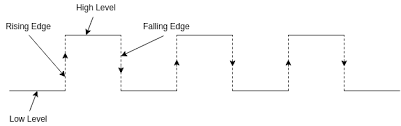
\includegraphics[width=0.8\textwidth]{download.png}
            \label{fig:my_label}
        \end{figure}
        \pause
        \item Use Master-Slave JK Flip-Flop
    \end{enumerate}
\end{frame}

\end{document}